\section{Vektorer} \label{mat:sec:vektorer}
Indtil nu har vi kun set på endimensionelle bevægelser, men som de fleste ved, sker langt fra alle bevægelser langs en linje. Når en bevægelse foregår i mere end én dimension, beskriver vi positionen med en \emph{vektor}.

En vektor er et matematisk objekt, der både har en retning og en størrelse.
Man tegner normalt vektorer som pile, og af denne grund angives de  her som $\va{v}$, hvor pilen over bogstavet viser, at det er en vektor. I fysik er det almindeligt, at angive vektorer med fed skrift, hvorfor det også gøres her.
Ligesom man kan lægge tal sammen, kan man også lægge vektorer sammen.
At lægge vektorer sammen svarer til at sætte dem i forlængelse af hinanden,
dvs. at summen af de to vektorer er den vektor, der går fra starten af den ene til slutningen af den anden, når den anden vektor starter ved slutningen af den første. Dette er illustreret på \cref{mat:fig:vekadd}, hvilket gør det noget tydeligere, end det er i ord.
Man kan også gange en vektor med et tal (en \emph{skalar}), hvilket forlænger eller forkorter vektoren med denne faktor. En negativ faktor vil således skifte vektorens retning.
Når vi lægger vektorer sammen eller ganger dem med tal, gælder alle de regneregler vi er vant til fra de reelle tal (tallene på en tallinje).

\begin{figure}
    \centering
    \begin{tikzpicture}[line width=2.5pt, scale=0.84]
        \coordinate (a) at (3.5,4.25);
        \coordinate (b) at (5.6,1.5);
        \coordinate (o) at (0,0);
        %
        \draw [dashed, line width = 1.75pt, blue] (a) to ++(-4,0);
        \draw [dashed, line width = 1.75pt, blue] (a) to ++(0,-4.55);
        \draw [dashed, line width = 1.75pt] ($ (a) + (b) $) to ++(-9.55,0);
        \draw [dashed, line width = 1.75pt] ($ (a) + (b) $) to ++(0,-6);
        %
        \draw [-{Stealth[length=4mm, width=2.5mm]}] (o) to (10,0);
        \draw [-{Stealth[length=4mm, width=2.5mm]}] (o) to (0,6.55);
        %
        \draw (9.9,-0.1) node[anchor=north]{\huge $x$};
        \draw (-0.1,6.4) node[anchor=east]{\huge $y$};
        %
        \draw [-{Stealth[length=4mm, width=2.5mm]}, red] (o) to ++($ (a) + (b) $);
        \draw [-{Stealth[length=4mm, width=2.5mm]}, blue] (o) to (a);
        \draw [-{Stealth[length=4mm, width=2.5mm]}, blue] (o) to (b);
        \draw [-{Stealth[length=4mm, width=2.5mm]}] (a) to ++(b);
        %
        \draw [red] ($ (a) + (b) $) node[anchor=south west]{\huge $\va{c} = \va{a} + \va{b}$};
        \draw [blue] (1.5,2.55) node[anchor=center]{\huge $\va{a}$};
        \draw [blue] (5,0.85) node[anchor=center]{\huge $\va{b}$};
        \draw (5,4.2) node[anchor=center]{\huge $\va{b}$};
        \draw [red] (7.5,4.2) node[anchor=center]{\huge $\va{c}$};
        %
        \draw [blue] (1.5,-0.45) node[anchor=center]{\huge $a_x$};
        \draw [blue] (-0.45,2.5) node[anchor=center]{\huge $a_y$};
        \draw (6.5,-0.45) node[anchor=center]{\huge $b_x$};
        \draw (-0.45,5) node[anchor=center]{\huge $b_y$};
        \draw (4.5,5.75) node[anchor=south]{\huge $c_x = a_x + b_x$};
        \draw (9.1,2.5) node[anchor=west]{\huge $c_y = a_y + b_y$};
    \end{tikzpicture}
    %
    % 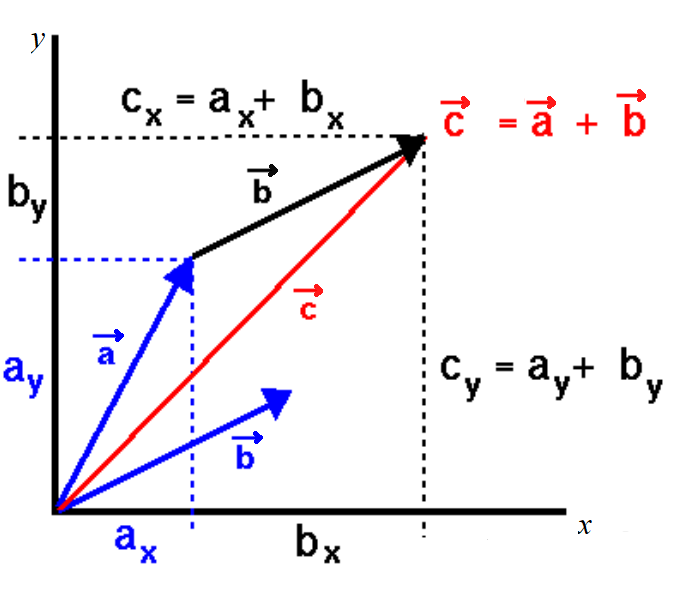
\includegraphics[width = 0.8\textwidth]{Matematik/matfig/vektoraddition.png}
    \caption{Illustration af vektoraddition, både grafisk og som komposanter. Den sorte og den blå vektor, der begge har navnet $\va{b}$ er den samme -- de er blot tegnet to forskellige steder i koordinatsystemet. Figuren er baseret på en figur fra \cite{VectorAddition}.}
    \label{mat:fig:vekadd}
\end{figure}

Når vi arbejder med vektorer i praksis, er en retning og en størrelse ikke altid super brugbart.
Derfor deler man vektoren op i \emph{komposanter}. 
Komposanterne er vektorer, der ligger langs akserne, som lagt sammen, giver den oprindelige vektor.
%
\begin{align}
    \va v = \va v_x + \va v_y = \begin{pmatrix}
    v_x \\ v_y
    \end{pmatrix}
\end{align}
%
Her er $\va{v}_x$ den del af vektoren $\va{v}$, som peger i $x$-retningen, og den har længden $v_x$. Tilsvarende gælder for $\va{v}_y$. Når man lægger vektorer sammen sker det komposantvist.
%
\begin{align}
    \va v+\va u=\va v_x+\va v_y+\va u_x+\va u_y= \begin{pmatrix}
    v_x+u_x \\ v_y+u_x
    \end{pmatrix}
\end{align}
%
Når vi ganger vektorer med et tal, er det som at gange ind i en parentes, og alle komposanterne skaleres på samme måde
%
\begin{align}
    a\va v=a(\va v_x+\va v_y)=a\va v_x+a\va v_y= \begin{pmatrix}
    av_x \\ av_y
    \end{pmatrix}.
\end{align}

Man skriver normalt længden af en vektor med lodrette streger på hver side af vektoren, $\abs{\va{v}}$ eller blot som vektoren symbol, som når vi skriver tal, $v$. 
Når man skal finde længden af en todimensional vektor, bruges Pythagoras' sætning
%
\begin{align}
    v^2 &= \abs{\va v}^2 = v_x^2+v_y^2. \label{pythagoras2}
\end{align}
%
Længden af vektoren $\va{v}$ er derfor
%
\begin{align}
    v &= \abs{\va{v}} = \sqrt{v_x^2+v_y^2}. \label{pythagoras2.5}
\end{align}
%
I tre dimensioner har vi tilsvarende at
%
\begin{align} \label{pythagoras3}
    v = \abs{\va v} = \sqrt{v_x^2+v_y^2+v_z^2}.
\end{align}
%
Længden af en vektor er altid positiv.
En særlig type vektor er dem, hvis længde er 1 -- de kaldes enhedsvektorer.
Vi skriver dem normalt med en hat\footnote{I gymnasiet har du måske mødt hatten som notation for en tværvektor. Tværvektoren giver dog kun mening i to dimensioner, og det bruges ikke i fysik. Til gengæld bruges hatten meget ofte til at symbolisere en enhedsvektor, hvorfor vi også vil bruge den notation.}; $\vu{v}$. Man kan altid danne en enhedsvektor ved at dele vektoren med sin længde\footnote{Når længden ikke er nul.};
%
\begin{align} \label{mat:eq:enhedsvektor}
    \vu{v} &= \frac{\va{v}}{\abs{\va{v}}} = \frac{\va{v}}{v}.
\end{align}
%
Man kan lave en enhedsvektor ud af enhver vektor\footnote{Undtagen nulvektoren, da man stadig ikke må dele med 0.}, men dem der ligger langs de kartesiske akser ($x$, $y$ og $z$) er særligt interessante. Disse vektorer kaldes basisvektorer, og skrives: $\vu{x}$, $\vu{y}$ og $\vu{z}$.
Det er engang imellem en fordel at skrive en vektor som en skaleret sum af basisvektorer
%
\begin{align}
    \va{v} &= v_x\vu{x} + v_y\vu{y} + v_z\vu{z}.
\end{align}

Når vi skal beskrive den tredimmensionelle bevægelse erstatter vi stedfunktionen $x(t)$ med en stedfunktionsvektor, $\va{r}(t)$, hvis komposanter opfører sig præcis som havde det blot været endimensionel bevægelse.
%
\begin{align}
    \va r(t)=\begin{pmatrix}
    x(t)\\y(t)\\z(t)
    \end{pmatrix}.
\end{align}

Nu mangler vi kun en ting for at kunne beskrive mekanikken i 3 dimensioner -- differentiering.
For almindelige funktioner var differentialkvotienten hældningen imellem to punkter, når vi lod de to punkter gå imod hinanden. Det samme kan også gøres for vektorfunktioner:
%
\begin{align}
    \dv{\va{f}}{t} = \lim_{\Delta t\rightarrow 0} \frac{\va{f}(t+\Delta t) - \va{f}(t)}{\Delta t}
\end{align}
%
Da der er essentielt tale om en forskel, hvilket sker indgangsvist for vektorer, foregår differentiation af vektorer også indgangsvist:
%
\begin{align}
    \dv{\va v}{t} = \begin{pmatrix} \dd v_x/\dd t\\\dd v_y/\dd t\\\dd v_z/\dd t\end{pmatrix}
\end{align}
%
Nu kan vi skrive Newtons anden lov som
%
\begin{align}
    \va{F} &= m \va{a} =m \dv[2]{\va{r}}{t},
    %
    \intertext{hvilket dækker over de tre ligninger}
    %
    F_x &= ma_x = m\dv[2]{x}{t}, \nonumber \\
    F_y &= ma_y = m\dv[2]{y}{t}, \nonumber \\
    F_z &= ma_z = m\dv[2]{z}{t}. \nonumber
\end{align}

Nu kunne man jo godt spørge sig selv: Når man kan gange vektorer med tal, kan man så gange dem med hinanden?
Svaret er ``ja''.
Der er faktisk to måder at gøre det på.
Den første er \emph{prikproduktet}\footnote{Kaldes også for skalarproduktet eller det indre produkt.}, der altid resulterer i et tal.
Her ganger man indgangene med hinanden, hvorefter man lægger det hele sammen, så
%
\begin{align}\label{mat:prikprodukt}
    \va{v} \cdot \va{u} = u_xv_x + u_yv_y + u_zv_z.
\end{align}
%
Det kaldes prikproduktet, fordi man angiver det med en prik.
Tager man prikproduktet af en vektor med sig selv genfinder vi vektorens længde i form af \cref{pythagoras2.5} eller \cref{pythagoras3}.
Mere generelt gælder det at
%
\begin{align}
    \abs{\va v\cdot \va u}=\abs{\va v}\abs{\va u}\cos(\theta),
\end{align}
%
hvor $\theta$ er vinklen imellem de to vektorer.
% $\cos$ står for cosinus og er en funktion fra trigonometrien.
Har man en retvinklet trekant, er cosinus længden af hypotenusen (den længste side) delt med længden af den hosliggende katete (den af de korte sider der danner vinkelen med hypotenusen), \cref{mat:eq:cos}.
Er vektorerne parallelle, er deres prikprodukt produktet af deres længder, siden $\cos(0)=1$.
Er vektorerne vinkelrette er prikproduktet nul, da $\cos(\ang{90}) = \cos(\pi/2) = 0$.
%Prikproduktet fortæller os således i hvor stor grad to vektorer er vinkelrette, hvilket vi kan bruge til at lave projektioner
%\begin{equation}
%    \text{Proj}_{\va u}(\va v)=\frac{\va v\cdot\va u}{\abs{\va u}^2}\va u=\frac{\va v\cdot\va u}{u^2}\va u
%\end{equation}

Det andet produkt er {\em krydsproduktet}\footnote{Kaldes også for vektorproduktet.},
der er defineret som
%
\begin{align} \label{mat:eq:krydsprodukt}
    \va{v} \times \va{u} =
    \begin{pmatrix}
    v_x\\v_y\\v_z
    \end{pmatrix}
    %
    \times
    %
    \begin{pmatrix}
    u_x\\u_y\\u_z
    \end{pmatrix}
    %
    =
    %
    \begin{pmatrix}
    v_yu_z-v_zu_y\\v_zu_x-v_xu_z\\v_xu_y-v_yu_x
    \end{pmatrix}.
\end{align}
%
Modsat prikproduktet giver krydsproduktet kun mening i tre dimensioner.
Grunden til at krydsproduktet er interessant, er at det giver en tredje vektor, der er vinkelret på de to første.
Krydsproduktet af to vektorer vil altid være vinkelret på dem begge. Er de to oprindelige vektorer parallelle vil den resulterende vektor være nul\footnote{Nulvektoren har nul i alle komposanter og er teknisk set vinkelret på alle vektorer.}.
For at finde retningen af et krydsprodukt bruges højrehåndsreglen (se figur \ref{mat:fig:right_hand_rule_mat}). Den er, at man lægger pegefingeren langs den første af de to oprindelige vektorer og langefingeren langs den anden, så vil krydsproduktet af de to ligge i tommelfingerens retning\footnote{Der er andre udgaver af højrehåndsreglen, men så længe man følger fingrene i samme rækkefølge, bliver resultatet det samme. Man kunne eksempelvis bruge tommelfingeren til første vektor og pegefingeren til den anden, hvorefter langefingeren giver retningen af krydsproduktet. Skifter man til venstre hånd får man et fortegnsskifte.}.
%
\begin{figure}[]
    \centering
    \begin{tikzpicture}[line width=2.5pt]
		\node[anchor=south west,inner sep=0] at (0,0)
		{ 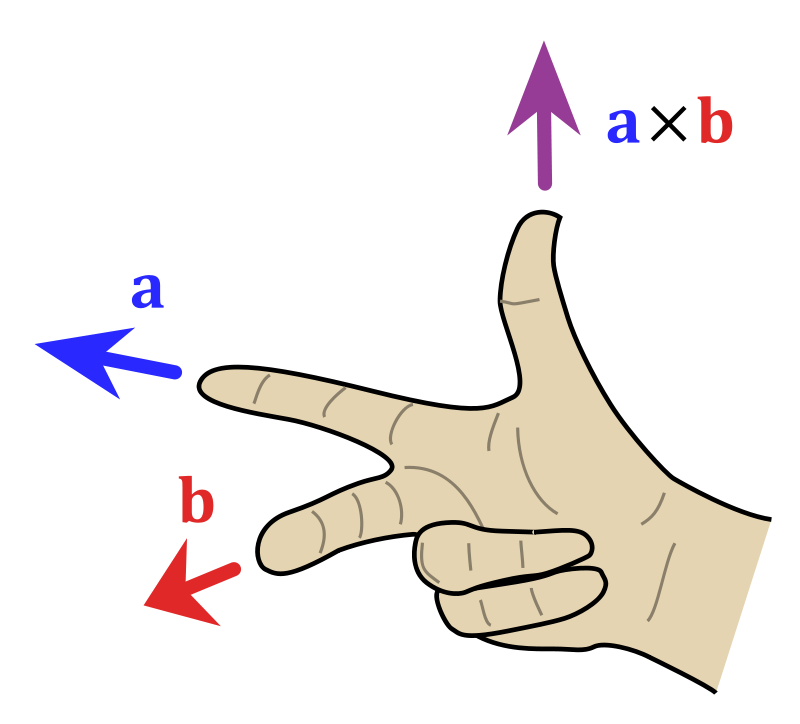
\includegraphics[width = 0.45 \textwidth]{Matematik/matfig/righthandmat.png} };
		% Nu indsættes hvide rektangler over originalteksten, som erstattes af vores egen
		\coordinate (a) at (1,3.6);
		\fill[white] (a) rectangle ++(1,1);
        \draw[blue] (a) node[anchor=south west]{\Huge $\va{a}$};
		%
		\coordinate (b) at (1.5,1.65);
		\fill[white] (b) rectangle ++(0.8,0.8);
        \draw[red] (b) node[anchor=south west]{\Huge $\va{b}$};
		%
		\coordinate (c) at (5.3,5.2);
		\fill[white] (c) rectangle ++(3,1);
        \draw[color=blue!50!red] (c) node[anchor=south west]{\Huge $\va{c} = \va{a} \times \va{b}$};
	\end{tikzpicture}
    % 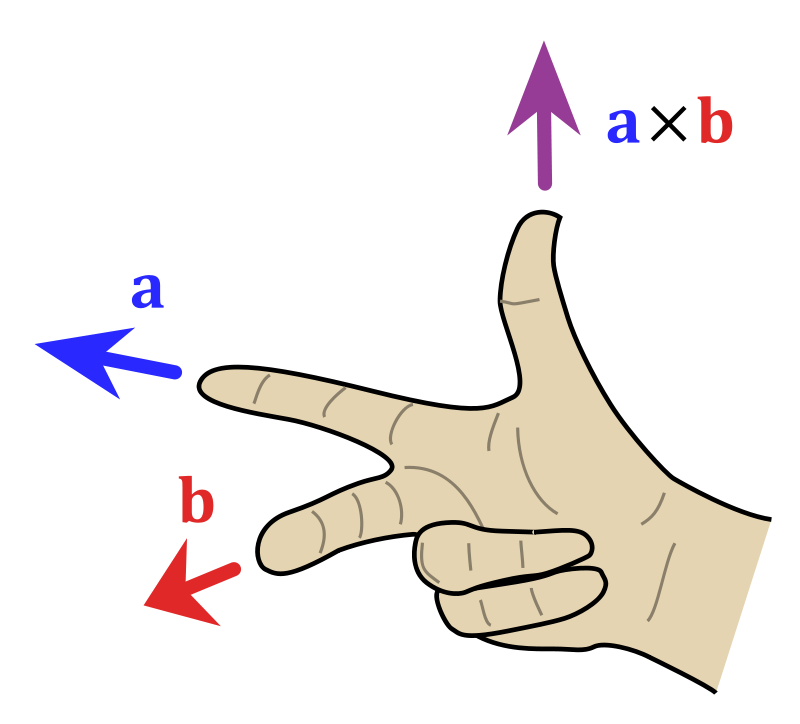
\includegraphics[width = 0.7 \textwidth]{Matematik/matfig/righthandmat.png}
    \caption{Højrehåndsreglen for retningen af krydsproduktet $\va{c} = \va{a} \times \va{b}$ imellem to vektorer $\va{a}$ og $\va{b}$. Figuren er en modificeret version af en fra \cite{RighthandRuleWikipedia}.}
    \label{mat:fig:right_hand_rule_mat}
\end{figure}
%
Længden af et krydsprodukt er
%
\begin{align}
    \abs{\va v \times \va u} &= \abs{\va v}\abs{\va u}\sin(\theta).
\end{align}
%
% $\sin$ står for sinus, der er en anden trigonometrisk funktion.
Hvor cosinus var forholdet imellem hypotenusen og den hosliggende katete, \cref{mat:eq:cos}, er sinus forholdet imellem hypotenusen og den modstående katete, \cref{mat:eq:sin}.
Modsat prikproduktet og almindelig multiplikation har rækkefølgen af de to vektorer i krydsproduktet en indflydelse på resultatet. Bytter man om på de to vektorer skiftes fortegnet:
%
\begin{align}
    \va v \times \va u &= -\va u\times \va v. \label{mat:eq:krydskommutator}
\end{align}
%
\Cref{mat:eq:krydsprodukt} kan være ret besværlig at bruge, så det er ofte lettere at dele udregningen op i enhedsvektorer. Krydsprodukterne af enhedsvektorerne er
%
\begin{subequations}
\begin{align}
    \vu{x} \times \vu{y} &= \vu{z}, \\
    \vu{y} \times \vu{z} &= \vu{x}, \\
    \vu{z} \times \vu{x} &= \vu{y},
\end{align}
\end{subequations}
%
og resten fremgår ved brug af \cref{mat:eq:krydsprodukt}.